\chapter{Inferring Interestingness of Tweets based on Information Flow Through the Network}


Mention:
\begin{itemize}
\item How this chapter builds upon network stuff in previous chapter
\item We hope to compare and contrast two better ways of predicting retweet volume \emph{and} interestness
\item What needs to be improved (speed, usability - more users with more followers etc.)
\item Why do improvements need to be made?
\item How is this useful, and how does first chapter relate to work done here?
\end{itemize}

Discuss:
\begin{itemize}
\item Does not use network to simulate tweets - instead uses a set of user features
\item Previous chapter shown how basic features can be used to generate a scale-free network, which is what twitter is
\item Use these features as input attributes of a new machine learning technique model.
\item This method does not use a network or model individual user decisions
\item Trained on a set of that particular user's tweets with the retweet outcome of integer type
\item A new tweet modelled with the regression outputs a retweet volume prediction without having to simulate the Tweet's travels through the network. 
\item Discuss about the machine learning approach used (logistic regression and how it works)
\item Talk about the 'binning' of retweet outcome volumes and its approaches (distribution dependent / independent, tables of precisions, etc.)
\item Link 'retweet volume' to 'retweet group size'
\end{itemize}

Research in the previous chapter focussed on researching the effect of the social graph on retweet propagation characteristics. From this, a methodology, displaying a range of various shortcomings, emerged based on the models and simulations utilised in the graph analyses. In this chapter, the methodology is modified with the aim of improving its performance and increasing the range of use-cases it is appropriate for. Since the social structure was found to play an important role in propagation, many network and user features are taken into account throughout the improvements.\\
In addition, modifications are made in order to provide an indication of \textit{how} interesting a piece of information is estimated to be, and more about this particular component is discussed in later sections.

The proposed methodologies also relate to the differences highlighted between a Tweet's raw popularity, as indicated by its retweet count, and hos interesting the Tweet actually is to those who read it. It has been shown that making retweet predictions against models trained with a large number of features can be accurate \cite{zhu11}, but in this work, the focus is more on the Tweet's content and beyond the static features.\\
That is, that when comparing Tweet popularity, then there may be some content, either within the Tweet itself or perhaps in a resource indicated by a URL contained in the Tweet, that makes the Tweet stand out to its recipients and to cause the aforementioned notion of \textit{affective stimulation} \cite{xu07} to its viewers.

Of course, this brings about the notion of information \textit{relevance}, and the fact that the same Tweet could be very boring or irrelevant to one user, and very interesting to another. In this work we focus on \textit{global} (or `average') interest, where interestingness inferences are made for the general case. It is considered that Tweets that are retweeted more than expected within their authors' local networks, relative to the usual retweet count of the authors' other Tweets, are also likely to be of interest to a wider audience, especially since they are now more likely to penetrate through the social graph enough to be received by users in different communities..
 
As such, the focus of the work in this chapter is that of adapting the inference methodology in order to develop a technique for accurately \textit{quantifying} the interestingness of tweets. This is concerning universal relevance in terms of highlighting interesting Tweets from the noise. In particular, there are two main improvements of the previous methodology to be made;
\begin{itemize}
    \item Improve method for generating the \textit{expected} retweet count of a Tweet (in terms of accuracy and range of application)
    \item Expand the binary retweet interesting inference into a more useful scale in order to support \textit{ranking} of interesting information.
\end{itemize}


\section{User Influence}
As has previously been posited, of importance to this work is the difference between the retweet count of a Tweet and the interestingness of the Tweet. An example in the Background chapter was provided, which related to the case of Justin Bieber. His account, \texttt{@justinbieber}, is one of the most influential on Twitter, with nearly 50 million followers at the time of writing. His Tweets receive an average of around 50-120 thousand retweets per Tweets, and they rarely receive fewer than 40,000 retweets.\\
Since an average Twitter user would generally attract a maximum of a few hundred followers, and would normally receive very few, if any, retweets per Tweet. A particularly interesting Tweet from such a user may be retweeted, for example, between 5-20 times. It is therefore apparent that, in the general case, an uninteresting Tweet from an influential user may receive 50,000 retweets, and an exceptionally interesting Tweet from a less-influential user may be retweeted 30 times. It is therefore clear that user influence dictates that this value cannot alone be indicative of Tweet interest.

However, since interestingness \textit{does} have an effect on an a user's individual retweet decision, this absolute retweet count can be used as part of the method for generating an interestingness \textit{score} for a Tweet.


\section{Interestingness Scores}
To address the notion of interest quantification, a scoring scheme is hereby introduced, allowing certain interesting Tweets to be ranked as `more interesting' than other interesting Tweets. This, in itself, is an improvement over the previous method, which allowed only for Tweets to be labelled as `interesting' or `non-interesting'.

Similar to the previous method's \textit{comparison} between the observed and expected retweet counts, the new scoring technique is based now on the \textit{difference} between the two counts. The general idea and potential use-case for this is that if a score is known for a set of Tweets, then these can be used as a basis for ordering information as part of information retrieval or an information delivery system, where Tweets can be displayed to users in a more useful way and where interesting Tweets could be brought forward to users who don't follow the source user or a retweeter, and thus deliver information to an interested user, yet without him or her having to know about it first.

Essentially, the notion scoring stems from the following scenario. Consider two Tweets, $A$ and $B$, which have the following properties;
\begin{itemize}
    \item $\ec{A} = 3000$ and $\rc{A} = 3010$
    \item $\ec{B} = 5$ and $\rc{B} = 15$
\end{itemize}
Where $\ec{A}$ represents the expected retweet count of $A$.

In this case, both Tweets would have been flagged as `interesting' under the previous scheme (although, in reality, the method would not be able to model users who are typically expected to achieve 3,000 retweets). However, it is clear that, despite the \textit{difference} between the counts being equal, Tweet $B$'s observed retweet count is actually much more significantly proportionately greater than what was expected, and is therefore likely to be more significantly interesting.

Since the proportionate difference is the key to this, the interestingness score, $\score{t}$, for Tweet $t$ is hereby simply given by;
\[
\begin{array}{cc}
 \score{t} = \frac{\ec{t}}{\rc{t}}
\end{array}
\]

This provides a positive score where;

\[
\score{t}
	\begin{cases}
		> 1		&	\text{indicates } t	\text{ is interesting} \\
		\leq 1	&	\text{indicates } t	\text{ is non-interesting}
  \end{cases}
\]

And where $\score{A} > \score{B}$ implies that $A$ is more interesting than $B$.

Since this methodology relies on data collection from Twitter in order to obtain the observed retweet counts, it involves extracting a snapshot of the state of the evaluated Tweets at one stage during their lifetime. Since Tweets are not removed over time, unless they are deleted by their author, they can be discovered and retweeted at any time after their composition and posting.\\
The work in this chapter assumes that the most significant portion of retweet activity for a specific Tweet has already occurred by the time the information on the Tweet has been collected. Indeed, the authors of \cite{kwak10} carried out investigative analyses into various temporal retweet brhaviours, and discovered that, on average, that a Tweet receives around 75\% of its retweets within the first day of being posted. 50\% of the retweets of a Tweet take place within the first \textit{hour} of the Tweet being posted.\\
Due to this, and to ensure that the retweet count collected is mostly representative of the Tweet's exraploated `final' retweet count, only Tweets that had been posted at least one day ago were considered for experimentation.


\section{Further Adaptations of the Inference Methodology}
In the previous chapter, it was noted how it was necessary to improve the method used for producing a Tweet, $t$'s, expected retweet count, $\ec{t}$. Problems with the previous method dictated that the method could only work under certain restrictions. In particular, that the user must have a small enough local network (in practice, a follower count of more than 500 or so made the method very unsuitable), and that, due to this, Tweets only attracting very few retweets could effectively be simulated. In addition, the interestingness inferences made were not significantly accurate, although this is likely due to a combination of the aforementioned issue providing much less room for error and the fact that the interestingness decision was only binary.

A new method is hereby proposed for carrying out the prediction for the value of $\ec{t}$. This method is immediately more superior to the previous, as only a very small amount of data (if any) is required to be collected from Twitter. This means that inferences on Tweet interestingness could be made on demand\footnote{Not `live' due to retweet action relies on time to occur.}.\\
Essentially, the method involves creating a classifier model capable of producing a base-line expected retweet count for a given Tweet and its relationship with its author. In this case, the classifier would be trained with the Tweet's actual retweet \textit{count} instead of the binary retweet decision used previously, and it would not require the simulations of the user's local network. Many more features regarding the Tweet, and its conetent, and its author are used to represent the particular user-Tweet information required for generating the predictions.

Since the graph structure clearly has an impact on message propagation, then it was felt that a significant consideration should be made towards including features relating to the interconnection of users, such as follower counts, Tweet rate, and information on a sample of friends and followers. More detail on the features used is provided in later sections.

In general, the newly proposed methodology follows these basic steps:
\begin{enumerate}
    \item Collect sufficent data from Twitter to train a classifier with an appropriate set of features. The trained model is known as the `global' model;
    \item Obtain a Tweet, $t$, and extract its own features as well as information about its author and its author's network properties;
    \item Classify the Tweet's features against the trained classifier to produce a retweet count prediction, $\ec{t}$ for this feature instance;
    \item Calculate \score{t} through using this $\ec{t}$ value and the known $\rc{t}$.
\end{enumerate}

In addition to this `global' model, a `user' model was proposed to be built for each user being evaluated. This user model would be much smaller, as it would only contain information on that user's historical Tweets, but would be capable of providing a second value for $\ec{t}$. With two such values, two scores could be generated by comparing the static $\rc{t}$ to each in turn.

As such, the two scoring mechanisms work as follows;
\[
    \gscore{t} = \frac{\rc{t}}{\ec{t}_1}
\]
\[
    \uscore{t} = \frac{\rc{t}}{\ec{t}_2}
\]


\section{Retweet Volumes as Nominal Attributes}
Most machine learning classifiers are not useful in accurately predicting the outcome of a feature of a large-ranging and continuous data type. Instead, the performance can be greatly improved when predicting from a limited range of discrete ranges, or `nominal' data.

Thus, in order to help improve the accuracy of $\ec{t}$ predictions, it was decided to convert the retweet count feature into a nominal data type for the purposes of training the model and making classifications. By `binning' the retweet counts into categories representing interval ranges, there would be fewer outcome possibilities, and thus the \textit{confidence} of classifcation could be greater.

The values for $\score{t}$ would then be determined through the ratio of $\rc{t}$ to the upper-bound of the nominal range category containing $\ec{t}$.


\subsection{Binning the Retweet Counts}
Since a trained classifier is only generally able to make predictions on features and values it has prior knowledge of, the bin ranges for each category must be equal in both the training feature data and the testing feature data. If the available nominal values for an instance feature representing a Tweet has a different set of category ranges to that in the trained classifier model, then it is likely that a prediction cannot be generated for this instance. It was therefore necessary to consider this when determining a method for binning the retweet counts.

There are various ways in which the counts could be binned, and all begin with a decision on the number of bins to use. The varying performance of this factor is considered later.

Initially, retweets were binned in a \textit{linear} fashion. That is, that the full range of retweet counts in the training set was calculated and then split into bins such that each category had an equal a range as possible. If there were no cases where $\rc{t} = 0$, then a category representing $[0,l)$, where $l$ is the minimum value for the lowest range, was pre-pended to the set of available nominal categories. Similarly, in all cases, the interval $[m+1,\infty)$ was appended to the set of categories, where $m$ is the maximum value in the highest range. This dictates that no Tweet in the training set can have a value for $\rc{t}$ in this category, and thus this allows any Tweet to potentially have $\score{t} > 1$. For example, if a training set of Tweets had a total range of values for $\rc{t}$ being between 1 and 20 was binned into four ranges, then the following interval categories would be applicable:
\[
    [0,1) [1,6) [6,11) [11,16) [16,21) [21,\infty)
\]

Since the distribution of retweet counts (expressed through retweet group sizes) is known \cite{webberley11}, then it is clear that this binning methodology would produce bins containing a very non-uniform distribution of Tweets, where the lower bin ranges would contain many Tweets and the cardinality of each category would decrease exponentially as the ranges become higher. This means that there would be fewer feature instances representing Tweets with larger retweet counts.\\
 Indeed, when training classifiers and running cross-validations on these, this binning scheme demonstrated a high accuracy of predictions on Tweets with lower values for $\rc{t}$ and a low accuracy for Tweets with higher counts. It would be more appropriate, and better address the desire for more universal use-cases expressed earlier in this and the previous chapter, if the accuracy of predictions could be more uniform across the bin ranges.

Various other methodologies were implemented, which eventually evolved into a histogram-based responsive  binning algorithm. Essentially, this algorithm involved is based around the initial calculation for the projected size of each bin, which is based on the total number of Tweets to be categorised and the target number of bins. Each bin was then filled according to the interval range specifying the bounds of that bin, and in such a way such that each retweet count frequency would only be present in one bin. For example, all of the retweets achieving one retweet would be placed in the single bin encompassing this value.\\
As such, after the intervals representing the bin bounds have been produced, then these represent the nominal categories for the retweet count feature in each instance for training and testing against the classifier.



\newfloat{algorithm}{H}{lop}
\begin{algorithm}
\caption{Algorithm for producing intervals for bin categories for $\rc{t}$ values.}
\begin{algorithmic}[1]
\Procedure{generate\_intervals}{set of Tweets $T$, number of bins $B$}
    \State $C\gets$ empty list \Comment{To hold ordered retweet counts}
    \State $I\gets$ empty list \Comment{To hold bin range intervals}
    \ForAll{$t \in T$}
        \State Add $\rc{t}$ to $C$
    \EndFor
    \State Sort $C$ into ascending order 
    \State $M\gets\max(C)$ \Comment{Highest instance of $\rc{t}$}
    \State $T\textrm{Sum}\gets\frac{|C|}{B}$ \Comment{Number of Tweets in each bin}
    \State $H\gets$ empty dictionary \Comment{Histogram of retweet count distribution}
    \Statex
    \ForAll{$c \in C$}
        \If{$c \in H$}
            \State Increment $H_c$
        \Else
            \State $H_c\gets0$
        \EndIf
    \EndFor
    \ForAll{$i$ in range $M+1$}
        \If{$i \in H$}
            \State $s = s + H_i$
        \EndIf
        \If{$s \geq T\textrm{Sum}$}
            \State Add $i$ to $I$
        \EndIf
    \EndFor
    \State Return $I$
\EndProcedure
\end{algorithmic}
\label{algo2}
\end{algorithm}
 
This new responsive method more readily supports more uniform bin sizes, and copes with this by expressing exponentially larger bin \textit{ranges}. As such, the distribution of bin sizes is generally described by a distribution simular to that shown in Figure \ref{fig:bin-hist}. As with the linear method, the interval $[0,l)$ is pre-pended, where necessary, and $[m+1,\infty)$ is always appended in addition to the intervals produced by the algorithm.

\begin{figure}[h]
\centering
\begin{tikzpicture}
\begin{semilogyaxis}[
    symbolic x coords={[0-1), [1-2), [2-3), [3-4), [4-5), [5-100)},
        ylabel=Cardinality of bin,
		xlabel=Bins,
        ybar,
        bar width=7pt,
        yticklabels={,,},
        xticklabels={,,}
        ]
   \addplot[plot 0,bar group size={0}{1}]
        coordinates {([0-1),100) ([1-2),50)  ([2-3),50) ([3-4), 50) ([4-5), 50) ([5-100), 25)};
        
\end{semilogyaxis}
\end{tikzpicture}
\caption{Example distribution of retweet count bin cardinalities under the responsive binning algorithm}
\label{fig:bin-hist}
\end{figure}

This method is responsive in that the bin ranges adapt to the variety and number of retweet counts available, and always attempts to produce a similar number of bins to what is requested. However, due to the disproportinately large number of small retweet groups, the bin sizes cannot be entirely uniform and means that the number of intervals returned will be smaller than the number requested.\\
This also stems from the fact that a single retweet count cannot exist in more than one bin concurrently; for example, if the interval $[0,2)$ existed in a scenario, and the number of Tweets with retweet count equal to 0 or 1 is greater than the value for $T\textrm{Sum}$, which is often the case, then this will result in a larger bin. Without this particular feature, a Tweet may be categorised into more than one bin, causing the prediction accuracy to be reduced. 

Due to this dynamicity, the bin ranges and cardinalities produced by the algorithm vary across different datasets. As a result, the nominal bin categories generated for producing the value for $\uscore{t}$ from the user model trained from the complete set of collected Tweets posted by $\aut{t}{O}$ would be different from those categories generated for a different user. The intervals in each bin category are therefore reflective of the various different number of retweets that each author's Tweets are likely to receive. 


\section{`Twitter is a Memepool'}
In 1976, Richard Dawkins coined the term `meme' to be defined as a ``unit of cultural transmission'' \cite{dawkins76}. The general idea behind memetics is as an analogy to biological genetics except, unlike genes, memes are entirely non-physical and represent a cultural idea or aspect or another human-based behaviour. The rise of social networks on the Internet has allowed the spread of memes to grow to the extent that they are sometimes now even \textit{represented} by physical constructs, such as images.

In genetics, a gene is a physical entity containing information and instructions. It is a unit of genetic inheritance, in that they are passed from parent to offspring through the act of reproduction, and the result of an organism having a gene will express the features represented by that particular gene. These genes contain instructions that make up the features of an individual, such as physical characteristics like eye colour and height, and non-physical characteristics, including various aspects of personality.\\
Organisms exist in an evironment that also has features, such as humidity, altitude, temperature, relations to other organisms, and so on. If the genes of an organism are such that they cause the individual to be well-suited to its environment, then that organism has a better chance of survival and, therefore, a better chance of achieving reproduction.

Memes are similar in that they are effectively made up of a set of features, or `memome', such as the wordings of a particular phrase, or their relevance to other cultural aspects. These enable the meme to be less or more likely to be replicated in different environments, which is made up of the humans exposed to it and the interactions between them. For example, an Internet meme relating to the Star Wars movies would likely have a greater chance of being reproduction, through discussion and reposting, in an environment comprising a set of science-fiction fans than when amongst more mixed-interest groups.

The meme is also a useful analogy in this thesis when describing the way in which Tweets undergo replication within Twitter. Like a meme, a Tweet has a specific set of features, such as the text it contains, the inclusion of any mentions or a URL, and so on, and it exists within an environment consisting of a set of interconnected users on the Twitter social graph.\\
A particular Tweet would generally have a greater chance of `surviving' and being replicated, through the act of retweeting, amongst certain users intereconnected in a particular way than in other environments.

As such, the Tweet features are analogous to the \textit{genes} of a genome, and the arrangement and type of users on the social graph that receive the Tweet and have an opportunity to assist in its propagation comprise the Tweet's \textit{environment}. Since the environment has previously been found to have a large effect on propagation, then these features are useful aspects to include as part of the improved methodology covered in this chapter.


\section{Generating Values for $\ec{t}$}
In order to generate the estimated retweet counts, a trained machine learning classifier is needed to make predictions on a set of feature instances. This section covers an overview of the classifier used for this purpose including a justification in terms of an analysis of its performance.


\subsection{Machine Learning Classifier}
An overview of machine learning classifiers and their processes was provided in the previous chapter. In that case, a logistic regression was used to generate a prediction on a binary retweet decision based on a small number of features. If the retweet count for the Tweet being trained or tested was greater than zero, then the retweet decision would be positive (\textsc{True}). Otherwise, the decision was negative (\textsc{False}).

Presently, the new methodology involves the prediction of a retweet count category from a set of nominal values of greater cardinality than two. As mentioned, the instances of a particular Tweet and its evironment are categorised based on the value of the retweet count of the Tweet. Although this means that a degree of accuracy is sacrificed when training the classifier, it does mean that there are fewer categories for predictions on test Tweet feature instances, providing a higher confidence in each prediction made.

The Bayesian network machine learning classifier was elected for use for the purposes required in this chapter. Use of this classifier in the social media domain is more rare than other classifiers, such as those involving a regression or a decision tree, but was selected for the various reasons highlighted later in this section.

The Bayesian network is an unsupervised classifier since its learning algorithms do not simply determine the class of the outcome, the retweet count, from the attribute features alone \cite{friedman97}. Instead, a probabilistic graph is constructed based on the dependencies between the variables. The variable attributes form the nodes of the graph and edges between the nodes denote the dependencies (or lack thereof) between them.

Thus, in the case of this research, the various Tweet and envirnomental features, including the nominal retweet count, form the nodes in the Bayesian Network. When forming the graph through training, the dependencies and their probabilistic weightings are adjusted so that an expected value for the retweet count can then be `predicted' from the values of all the other variable attributes.


\subsection{Classification Performance}
When selecting classifiers, the Weka\footnote{http://www.cs.waikato.ac.nz/ml/weka} machine learning and data mining toolkit was used to evaluate the relative performance of various types of appropriate classifiers for the task. The classifiers were selected to cover a sample of the range of available classifier categories. Whilst some types may work inefficiently in this scenario, it is likely that they are more efficient when employed in different use-cases.\\
Although the accuracy of prediction was important, it would also be useful for the classifier to be \textit{efficient} in training its model and when testing future instances against it. This is so that this method could be used to produce interestingness inferences on demand and to further improve on the methodologies used in the previous chapter.

\begin{table}[h]\footnotesize
\begin{center}
\begin{tabular}{ l | c | c | c }
	Classifier	& Precision & Accuracy (recall) &  training time (secs.) \\
	\hline
	\hline 
	Simple logistic & 52\% &  56\% & 528\\
    Logistic        & 62\% &  56\% & 18\\
    SMO             & 51\% &  55\% & 1384\\
    Na\"{i}ve Bayesian & 50\% & 44\% & 0.13\\
    Bayesian network & 62\%&  64\% & 0.54\\
    \hline  
\end{tabular}
\end{center}
\caption{The training performance of different machine learning classifiers.}
\label{table:classifierperformance}
\end{table}

The Bayesian network was found to be accurate and time efficient when evaluating the performance of the set of classifiers. A dataset, obtained as part of the general data collection (please see the relevant section below) and which contains a set of over 57,000 Tweets, was identically used in each of the analyses. For each Tweet instance the same retweet count binning scheme was used, and each classifier performed the same number of cross-validations against the same dataset in order to obtain the precision and recall values.

Although the dataset used in this analysis is not the complete set used in practice, the cardinality of the dataset was sufficient to cause the outputs to be indicative of the Bayesian network's relative advantages over the other assessed classifiers.


\subsection{Varying the Cardinality of Nominally-Categorised Retweet Counts}
Applying the continuous retweet count values to produce a set of nominal categories representing interval ranges of the retweet counts requires a certain balance.\\
By reducing the number of target category bins then the classification accuracy increases, but the level of applicability of the eventual interestingness score for the wide range of retweet counts observed would be reduced. Inversely, with too many bins, the classification accuracy reduces, as there would be fewer instances in each category, yet the scores would be apliccable to a wider range of retweet counts.

\begin{table}[h]\footnotesize
\begin{center}
\begin{tabular}{ c | c | c | c }
	Target category count	& Resultant category count & Precision &  Accuracy (recall) \\
	\hline
	\hline 
    1 & 1 & 100\% & 100\% \\
    2 & 2 & 89.3\% & 89.3\% \\
    5 & 4 & 78.8\%  & 74.5\% \\
    10 & 7 & 68.6\% & 65.7\% \\
    15 & 10 & 61.2\% & 56.4\% \\
    20 & 12 & 59.1\% & 52.9\% \\
    25 & 15 & 51.4\% & 47.5\% \\
    30 & 18 & 49.3\% & 45.3\% \\
    35 & 21 & 47.2\% & 43.2\% \\
    40 & 23 & 46.2\% & 42.5\% \\
    \hline  
\end{tabular}
\end{center}
\caption{The effect of varying the number of nominal categories representing retweet counts on the classification performance using a Bayesian network classifier.}
\label{table:binperformance}
\end{table}

Clearly, by increasing the number of nominal categories used, then the relative number of feature instances in each eventual interval decreases. These bins represent the nominal categories that each feature instance is classified as in relation to the predicted retweet count of the instance. Table \ref{table:binperformance} outlines the decrease in classification accuracy observed with increases in target bin count. The dataset used consisted of nearly 67,000 Tweets, also as part of the ongoing general data collection discussed in later sections, and the classifier used to conduct the analysis was a Bayesian network through cross validation.

It has already been discussed that the resultant bin count is usually likely to be less than that requested of the binning algorithm. This is due to the long-tail distribution of retweet counts referred to previously.\\
In the coming experimentations the algorithm tried to produce, where possible, about 10 nominal ranges for use with training and testing against the general global dataset for the purposes of generating the global expected retweet count. Since each user's own retweet count ranges were different, the number of categories were calculated individually for producing the user-centric expected retweet counts as part of calculating values for $\uscore{t}$.


\section{Training and Testing Against the Bayesian Network Classifier}
This section discusses the processes used behind the calculation of interestingness scores for Tweets through the generation of expected retweet counts using the methodologies outlined in the previous sections. Particular focus is lended to the data collection and the features extracted through the resultant data corpora.


\subsection{Collecting the Training and Testing Data}
In order to train the model on a set of Tweets and then use it to make predictions, data was required for collection from Twitter. This data could then be divided up when required, as described below.

Since, in this case, it was necessary to collect the Tweet data along with each Tweet's numeric retweet count, rather than the binary nominal yes/no required in the previous chapter, only the retweets of a particular Tweet that had been created using the button method could be considered. This is because a Tweet's retweets executed using the manual copy and paste method do not contribute to the Tweet's official, and observable, retweet count that is returned from Twitter's API. This is not considered to be a limitation, however, since this factor is used consistently through the training and later evaluation of the trained model.

In March 2013, a random walk was conducted through Twitter's social graph using v1.1 of Twitter's REST API. Although this date was before the mandatory transfer to this version of the API, the crawler method was used in preference over collecting from the public API, which was deprecated and removed in v1.1, so that user data could be collected, as described, for the environmental training features.

The walk originated with one Twitter user, and each stage consisted of focusing on one user before selecting another one from the followers of the currently focused user. As such, the crawler is very similar to that used in the latter sections of the previous chapter.\\
At each step of the crawl, a set of the most recent Tweets authored by the current user were collected. The number of Tweets obtained for each user had various dependencies, such as the user's Tweet-posting frequency and the number of Tweets in total posted by the user. Usually, several hundredf Tweets from each user were yielded. In addition to the Tweet data, information on the user itself was collected as well as on a sample subset of up to 100, if they exist, of its friends and followers.\\
A sample subset of friends and followers was used instead of the complete set for the purposes of efficiency and to address the associated limitation in the previous interestingness inference methodology, yet it still provides an example snapshot of up to an additional 200 users in the author user's local network in order to provide some idea of the activity within the local network both upstream and downstream from the author user. Around ten API calls were required to obtain this information for each user, giving it immediate advantages over the older method. 

The data collection crawl resulted in a dataset containing around 241,000 Tweets authored by 370 unique Twitter users. Of those Tweets, around 90,000 were cases in which the retweet count was greater than zero. The partial datasets as subsets of the complete set, obtained up until various intermediate points of the entire collection, were those used by the classifier and binning performance analyses in the previous section.\\
Importantly, Tweets from many different types of user were collected; from less-active users with very few followers and friends to influential users and celebrities with millions of followers and achieving many thousand retweets. The collection of this range of users will help demonstrate if this new methodology is able to correctly assess a wider range of users and Tweets.


\subsection{Data Corpora}
After collection, the complete data was divided into two datasets; a training set, consisting of 90\% of the entire set, and a testing dataset, consisting of the remaining 10\%. The original set was divided in such a way as to ensure that all of the Tweets authored by one particular user existed in only one of the two resultant datasets. After being used to train the Bayesian network model, the larger dataset was then discarded from use for the rest of the experimentation.

As has been previously mentioned, of interest is the generation of \textit{two} interestingness scores for each Tweet, $t$; one based on a comparison between $\rc{t}$ and an $\ec{t}$ produced from the global model, and the other between $\rc{t}$ and an $\ec{t}$ produced from $\aut{t}{O}$'s user model. As such, each Tweet requires the two models in order to provide the predicted values for $\ec{t}$.\\
To assist with this, individual user datasets were extracted from the testing dataset, each containing information only on that particular user and its local network and its Tweets, from which individual user Bayesian network models could be trained.

The complete testing dataset is referred to as the `global' corpus of Tweets, and each individual user dataset is known as a `user' corpus.



\subsection{Features}
Producing the instances used for testing and training the Bayesian network models involved the extraction of various features from the global and user datasets. Generally, each feature falls into one of three categories; the network features (`environment'), the Tweet features (`genome'), and the author features (representing the author of the current Tweet). The nominalised retweet count is categorised as a Tweet feature.

Generally, the Tweet features follow the same notions as those used in the previous chapter in that they are static and generally binary features describing various aspects of the Tweet's content and metadata. The network features are more variable and describe the ways in which the author's local network is constructed and the activity within it.

Each Tweet is represented by an instance of a complete set of features relating to that Tweet, its author, and its author's local network. As a result, feature instances representing Tweets authored by the same user will share the same values for their network and author features.


\subsubsection{Features for the global corpus model}
The global corpus model is the Bayesian network model representing the classifier trained from the complete training dataset. In this case, a total of 31 features, outlined in Table \ref{table:globalfeatures}, were used to train the classifier.\\
As such, there were around 217,000 Tweet instances using this feature scheme used for traning the global classifier.

\begin{table}[h]\footnotesize
\begin{center}
\begin{tabular}{ c | l | c }
	 Feature category	& Feature & Feature data type \\
	 \hline
	 \hline 
	& mention & \{True, False\}\\
    & Tweet length & real (numeric)\\
    & url & \{True, False\}\\
  	& hashtag & \{True, False\}\\
  	Tweet & positive emoticon & \{True, False\}\\
  	(`genome')& negative emoticon & \{True, False\}\\
  	& exclamation mark & \{True, False\}\\
  	& question mark & \{True, False\}\\
  	& starts with `RT' & \{True, False\}\\
  	& is an @-reply & \{True, False\}\\
    & \textbf{retweet count} & \textbf{[dynamic nominal]}\\
  \hline                        
	& follower count & real (numeric)\\
    & friend count  & real (numeric)\\
	Author & verified account & \{True, False\}\\
	& status count & real (numeric)\\
	& listed count & real (numeric)\\
    \hline
  	&  max. follower count & real (numeric)\\
	&  min. follower count & real (numeric)\\
	& avg. follower count & real (numeric)\\
    Network & max. friend count & real (numeric)\\
	(`environment') & min. friend count & real (numeric)\\
	& avg. friend count & real (numeric)\\  
	& avg. status count & real (numeric)\\  
  	& proportion verified & real (numeric)\\  
  \hline  
\end{tabular}
\end{center}
\caption{Features used to train the model from the global data corpus.}
\label{table:globalfeatures}
\end{table}

The network features listed apply to both samples of the followers and friends retrieved for each author user during the data collection. For example, the first feature of this category, `max. follower count', represents two features referring to the maximum follower count observed across the sample of the user's followers and the sample of the user's friends respectively.

It should be noted that although the Tweet features, aside from the retweet count as has already been discussed, are permanent after the Tweet has been created and posted, the author and network features are more dynamic due to the continuous mutations in the social graph as edges representing followships are constantly being formed and broken between the user nodes. In this thesis, it is assumed that changes to the features representing these factors were not significant over the period of posted Tweets for each user, and the effect is minimised through consideration only of the recent Tweets of each author user.


\subsubsection{Features for individual user models}
Since the author and network features have identical values in the instances representing all of the Tweets from one particular user, then these features were not considered when training and testing using the user models.\\
As such, the 10 Tweet features were those used in the feature instances in training, and testing against, each user model.

 

\subsection{Testing Against the Trained Classifier}
Once the feature extraction was completed and the instances were built for the global training dataset and each individual user set, the models were trained as described above.

In order to produce the expected \textit{global} retweet counts, each Tweet $t \in T$, where $T$ represents the entire testing dataset, had its features extracted, less the retweet count nominal category, and was evaluated against the global model. This classified each Tweet into one of the categories given by that Tweet's predicted retweet count, and the top interval of the expected retweet outcome category became the \textit{expected} retweet count for that particular Tweet.\\
Similarly, the expected \textit{user} retweet counts were produced in the same way, but instead each Tweet was classified by the user model associated with that Tweet's author.

In each case, the two interestingness scores for each Tweet could be calculated, based on the process described earier, using the ratio between the Tweet's two expected retweet counts and its \textit{observed} retweet count stored as part of the data collection from Twitter. This meant that each Tweet $t \in T$ had two numeric scores, $\uscore{t}$ and $\gscore{t}$, assigned to it. 



\section{Initial Validations of the Scoring Methodologies}
Similar to in the previous chapter, tests are required in order to ensure the validity of the interestingness scores applied to each of the Tweets in the testing dataset. By running these validations, the relative performance of the scoring mechanism can be assessed, and the comparative performance of the two scores, $\uscore{t}$ and $\gscore{t}$ can be evaluated.


\subsection{Planning the Validations}
It was decided that crowdsourcing through Crowdflower and Mechanical Turk, again, would be used to validate the new scoring mechanism, as this would facilitate interestingness evaluations from a wider range of human input. The MTWs taking part would not be associated with the collected Tweets in any way, and thus this assists in the identification of the non-noisy Tweets that are `globally' interesting and are those that the scores have theoretically determined as `interesting'.

Certain Tweets and users were removed, at this stage, from the dataset of Tweets to be assessd by the MTWs. Since the Tweet data was collected through a random crawl through the Twitter and no checks were placed on the crawler at that stage, there was no governance over the content of the text in each Tweet of the data. Thefore, users who frequently used offensive phrases or wrote Tweets in non-English had their Tweets removed. The reasoning behind the latter is based on the fact that the Mechanical Turk microtasks were submitted to be completed by people living in the USA.\\
As before, individual Tweets that were `@-replies' were also stripped so that only Tweets intended to be broadcasts were included in the final MTW test set.


\subsection{Validating the Methodology Outcomes}
In the context of this validation scheme, the MTWs were random account-holders on Mechanical Turk and had no connection to the Tweets they were evaluating. By not determining the humans to make the assessments, a more diverse opinion on the interestingness can be achieved, as the different users will have varying considerations on what contstitutes `noise' and will therefore form a more diverse opinion and further reinforce a decision when multiple MTWs form agreements on what is interesting. 

The validations were carried out such that the MTWs were presented with a series of questions, each of which consisting of five different Tweets from \textit{one} specific author. As such, Tweets were assessed against others than had been posted by the same user. In each question, the MTWs were asked to select the Tweets that they consider to be the most interesting of the group, and that they must select at least one Tweet for each question. For each judgment, where a judgment is one question answered with one or more Tweets selected, MTWs were paid \$0.05.

The test was conducted under the condtitions of a randomised controlled trial. To this end, each Tweet was assessed in three different contexts, in that it would appear in three different questions alongisde four other randomly chosen Tweets, and that each question would then be judged by three different MTWs.

From the stripped testing dataset, 750 Tweets were selected, at random, to be filtered by the author user into the questions to be assessed on Mechanical Turk. Since each Tweet was to appear in three different questions and since each question consisted of five unique Tweets, then this resulted in a total of 450 different questions. Each of these questions was then judged by three different MTWs.


\subsection{Outcomes From the Validations}
The validation test involved contributions from 91 different MTWs, demonstrating the wide diversity of human input attainable validations employing crowdsourcing in this way. From these MTWs, 325 of the 450 questions in total asked had responses where a Tweet was selected with a confidence of two-thirds or greater. Since the MTWs had the opportunity to select more than one Tweet of each question to be the most interesting, there were 349 Tweets of the original 750 Tweets, denoted as $T' : T' \subset T$, that were selected as sufficiently interesting by the MTWs. Tweets selected from individual questions that did not have sufficient confidence were discarded.

The remainder of this section analyses the validation data in various ways to demonstrate the strengths and weakenesses of the interestingness score inferences.\\
Of immediate notice was the comparitive difference between the two different scoring mechanisms for each Tweet $t$; $\gscore{t}$ and $\uscore{t}$. The inference validation results are not significant between the use of the two scores in any of the analyses conducted. As such, the following analyses concern only the use of $\gscore{t} \forall t \in T'$.


\subsubsection{General Performance}

\begin{figure}[h]
\centering
\begin{tikzpicture}
\begin{semilogyaxis}[
    symbolic x coords={{[0,1)}, {[1,2)}, {[2,3)},{[3,4)}, {[4,5)}, {[5,100)}}, % inside braces to support commas in intervals
        ylabel=Proportionate frequency,
		xlabel=$\gscore{t}$,
        ymin=1,
        legend pos=north east,
        legend style={nodes=right},
        ybar,
        bar width=7pt,
        legend entries={ Chosen Tweets ($T'$),  All Tested Tweets ($T$)}
        ]
   \addplot[plot 0,bar group size={0}{2}]
        coordinates {({[0,1)},76.30057803) ({[1,2)},7.514450867)  ({[2,3)},4.335260116) ({[3,4)}, 1.445086705) ({[4,5)}, 2.023121387) ({[5,100)}, 6.936416185)};
        \addplot[plot 1,bar group size={1}{2}]
        coordinates {({[0,1)},80.94365552) ({[1,2)},6.596426935)  ({[2,3)},3.710490151) ({[3,4)}, 1.099404489) ({[4,5)}, 0.961978928) ({[5,100)}, 4.634448007)};
        
\end{semilogyaxis}
\end{tikzpicture}
\caption{Proportionate frequency distribution of $\gscore{t} \forall t \in T$ compared to only those $\gscore{t} \forall t \in T'$}
\label{fig:hist}
\end{figure}

Of the subset $T'$, the scoring mechanism found 140 of the Tweets to have a value of $\gscore{t} > 1$, and thus inferred as interesting. Of these, 65\% were agreed on as interesting by the MTWs. The performance of the $\uscore{t}$ was worse in providing a 55\% agreement, resulting in a general of 60\% agreement on the mean of the two scoring schemes.\\
It is also demonstrable that the proportionate frequency of Tweets with higher values of $\gscore{t}$ is greater in the subset $T'$ than in $T$. This implies that, on average, the MTWs were selecting and agreeing on Tweets being interesting that had a higher score than those that were \textit{not} selected. Further to this, there is a greater proportion of Tweets with lower scores ($0 \leq \gscore{t} < 1$) in $T$ than in $T'$, and a greater proportion of higher values for $\gscore{t}$ in $T'$ than in $T$.

This means that, in general, the humans were marking a greater number of Tweets as interesting that were inferred as interesting by the scores than ones that \textit{weren't} inferred as interesting. Although this demonstrates a clear advantage on the binary inference of interestingness over the methodologies in the previous chapter, this analysis does not consider how well the scheme is able to \textit{rank} Tweets in order of interestingness.


\subsubsection{Per-Question Performance}

In order to assess the ability of the scores to effectively rank Tweets in order of inferred interest \textit{level}, the Tweets were studied on a per-question basis.

\begin{figure}[h]
\centering
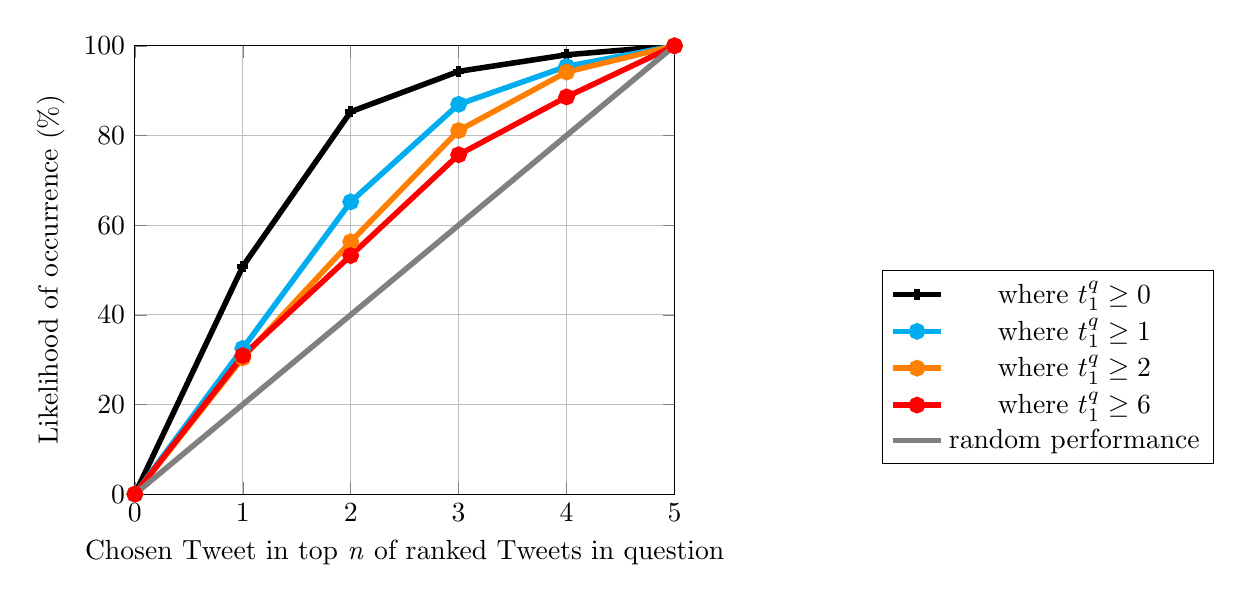
\begin{tikzpicture}
 \begin{axis}[
        xlabel=Chosen Tweet in top \textit{n} of ranked Tweets in question,
        ylabel=Likelihood of occurrence (\%),
        grid = major,
        legend entries={where $\gscore{t^q_1} \geq 0$, where $\gscore{t^q_1} \geq 1$, where $\gscore{t^q_1} \geq 2$, where $\gscore{t^q_1} \geq 6$, random performance},
		legend style={at={(2,0.5)}},
		xmin=0, xmax=5,
		ymin=0, ymax=100
		]
	\addplot[mark=+,black] plot coordinates {
        (0,0) (1,50.8) (2,85.3) (3,94.3) (4,98) (5,100)
        };
        
	\addplot[mark=*,cyan] plot coordinates {
        (0,0) (1,32.5) (2,65.2) (3,86.95) (4,95.4) (5,100)
        };
    \addplot[mark=*,orange] plot coordinates {
       (0,0) (1,30.4) (2,56.3) (3,81.1) (4,94.15) (5,100)
    };
    \addplot[mark=*,red] plot coordinates {
        (0,0) (1,30.9) (2,53.2) (3,75.7) (4,88.6) (5,100)
    };
    \addplot[gray] plot coordinates {
        (0,0) (1,20) (2,40) (3,60) (4,80) (5,100)
    };
\end{axis}
\end{tikzpicture}
\caption{The probability of a selected Tweet's $\score{t}$ being in the top \textit{n} of \textit{ranked} Tweets for that question. Also illustrating the effect of raising the minimum allowed $\gscore{t^q_1} \forall q \in Q$}
\label{fig:score-dist}
\end{figure}

These questions are those that were assessed by the MTWs and where a particular question, $q \in Q$, where $Q$ is the set of all 450 questions, is comprised of a set of Tweets such that $|q| = 5 \forall q \in Q$.\\
In order to conduct this analysis, each question $q$ had its five Tweets $t \in q$ ranked in order of ascending $\gscore{t}$, such that;
\[
    q = (t^q_1, t^q_2, t^q_3, t^q_4, t^q_5)
\]
and where; 
\[
    \gscore{t^q_1} \geq \gscore{t^q_2} \geq ... \geq \gscore{t^q_5}
\]
In cases where $\sum\limits_{i=1}^5 \gscore{t^q_i} = 0$, then that $q$ was removed from $Q$ and discarded for the analysis.

Calculations were then made on the number of times the MTWs selected a Tweet as interesting that appeared in the top $n$ of the ranked list Tweets for each $q \in Q$. For example, in the case of $n=2$ with a set of ten questions, if the MTWs selected one of the top two of Tweets in five of ten cases, then the chance of this occurring is 0.5. Figure \ref{fig:score-dist} illustrates the relationship between increasing values of $n$ and this calculation on likelihood of selection. Although the `random' performance represents the relative likelihoods of a random selection being made when only one Tweet is selected from each question, the vast majority of questions were actually answered with only one Tweet selected. Further analysis to cover the consideration of this particular point is conducted later on in this chapter.\\
Further to this, the minimum allowed value of $\gscore{t^q_1}$, which represents the highest score of all $t \in q$, was varied with the aim of demonstrating that the detection of more interesting Tweets can be more accurate when the relative score \textit{range} of a particular question is more disparate.

When considering cases where the most interesting Tweet in a particular question is, indeed, inferred as interesting ($\gscore{t} \geq 1$), then the MTWs selected one of the \textit{top two} Tweets in around 66\% of cases, and they selected one of the \textit{top three} ranked Tweets in 87\% of the questions. This demonstrates the method's ability of being able to effective rank Tweets in agreement with humans in identifying information from the noise around it.


\subsubsection{Probability of Selection}
A further analysis in this section is with regard to the \textit{probability} of a particular inferred-as-interesting Tweet being selected as interesting by the MTWs. It is demonstrable that that, in general, the chance of a particular MTW deciding that a Tweet, $t$, is interesting becomes greater as the value of $\gscore{t}$ increases.

\begin{figure}[h]
\centering
\begin{tikzpicture}
\pgfplotsset{every axis plot/.style={line width=2pt}}
 \begin{axis}[
        xlabel=$ x $,
        ylabel=$P(\text{t chosen} : \gscore{t} > x)$ ,
        grid = major,
        xmin=0, xmax=4
       ]
	\addplot+[smooth, mark=none]  table {5.Chapter3/data/cum-dist-score.dat};
\end{axis}
\end{tikzpicture}
\caption{Cumulative frequency representing the probability that Tweet $t$ is chosen provided that $\gscore{t}$ is greater than a given value, $x$}
\label{fig:score-cum-dist}
\end{figure}

Although the cases of Tweets where $\gscore{t} > 4$ are excluded, for the purposes of noise reduction from fewer samples, Figure \ref{fig:score-cum-dist} shows an observable increase in probability of selection as the score increases. This pattern is particularly applicable in the score interval of 0-1, which represents the range of Tweets that the scoring scheme has inferred as uninteresting to those that achieved a correctly-predicted popularity, and are thus `as expected' in terms of interestingness.\\
The analysis is also clear that Tweets with an inferred interestingness score of three or more are not significantly different from one another in terms of the level of interestingness assigned from the `real' human judgment.


\subsubsection{Discerning Interesting Information from Noise}
The metrics behind the human selection in determining interesting Tweets is the final analysis conducted in this section. Of particular concern is the varying likelihood of \textit{agreement} between the MTWs and the relative properties of the Tweets and their scores in each question in different decision scenarios.

The notion of score \textit{disparity} is used to determine the difference in interest between a set of Tweets presenting with a range of different interestingness scores. To this end, each question asked of the MTWs has a disparity associated with it. The absolute score disparity for a question, $q \in Q$, is calculated such that;
\[
    \gdisparity{q} = \max(\gscore{t}) - \min(\gscore{t}) \forall t \in q
\]

\begin{table}[h]\footnotesize
\centering
\begin{tabular}{ c | c | c | c }
	 Num. confident answers in $q$ & min. $\gdisparity{q}$ & max. $\gdisparity{q}$ & avg. $\gdisparity{q}$ \\
	 \hline
	0 & 0 & 846 & \textbf{17.6} \\
	> 0 & 0 & 1445 & 32.1 \\
	1 & 0 & 1445 & \textbf{34.3} \\
	> 1 & 0 & 4 & 0.647 \\
	> 2 & 0 & 0.55 & 0.204
\end{tabular}
\caption{Illustrating trends between the absolute $\gdisparity{q}$ with the varying number of confident answers made in $q$. Entries in \textbf{bold} are used to highlight interesting values}
\label{table:score_disparities}
\end{table}

A confident answer to a question is one where the particular question had at least two of its three assessing MTWs select the same Tweet as interesting. Since an MTW could select more than one Tweet from each question, then each question may, in fact, have more than one confident answer. Table \ref{table:score_disparities} illustrates how questions with varying score disparities can have an effect on the probability of MTWs being able to make a confident decision.

The results show that the average $\gdisparity{q}$ of all $q \in Q$ is roughly double in cases where a question is answered with precisely one confident Tweet than in cases where there was no confident answer made at all. This indicates that a wider range of interestiness of information is helpful to humans in identifying the content they'd prefer to read. If several pieces of information were displayed to a user that had more similar scores, and are therefore more equally interesting (or uninteresting), then it becomes more difficult for an agreement to be made between the different users on which particular piect of information is the \textit{most} interesting.

Further to this, the average disparity is much lower in cases where the question had multiple confident answers made. In these cases, the MTWs have selected more Tweets as interesting, which helps to reinforce the above point in that identifying one particular piece of information as the most interesting is more difficult when the pieces are all of similar interest levels. Indeed, in questions where this is the case, MTWs have selected, and agreed on, multiple Tweets. 

 \begin{figure}[h]
\centering
\begin{tikzpicture}
\pgfplotsset{every axis plot/.style={line width=2pt}}
 \begin{axis}[
        xlabel=Average $\gdisparity{q}$,
        ylabel=Cumulative probability,
        grid = major,
        ymax=1,
        ymin=0,
        xmin=0
       ]
	\addplot+[mark=none]  table {5.Chapter3/data/cum-question-disparity.dat};
\end{axis}
\end{tikzpicture}
\caption{Cumulative probability of a confident selection being made for question $q$ with varying $\gdisparity{q}$}
\label{fig:cum-question-disparity}
\end{figure}

Table \ref{table:score_disparities_2} highlights the effect of disparity on human selection also through demonstrating that in \textit{all} $q \in Q$, and not just those that have been confidently answered, the score disparity between all of the Tweets in a particular question that were selected, $\sdirparity{q}$, is much smaller than the general disparity of the entire question, $\disparity{q}$. In this case, the disparities are dependent on the particular scoring scheme declared in order to highlight the differences between the two scores, and where;
\[
    \ascore{t} = \frac{\gscore{t} + \uscore{t}}{2}
\] 

This feature is particularly observable in cases where a question consists of a few Tweets having similarly high scores amongst Tweets with collecively lower scores. Therefore, inferring the interesting Tweets is easier, demonstrated by the scores of selected Tweets being generally higher, but discerning one \textit{most} interesting Tweet is not as trivial. For example, the results show that, on average, the disparity of the global scores across selected Tweets is around 57\% of the disparity across \textit{all} of the Tweets in a particular question.


\begin{table}[h]\footnotesize
\begin{center}
\begin{tabular}{ l || c | c | c }
	   & $\gscore{t}$ &  $\uscore{t}$ &  $\ascore{t}$\\
	 \hline
	$\disparity{q}$ & 62.4 & 4.7 & 33.3\\
	$\sdisparity{q}$ & 35.3 & 3.1 & 19.0\\
	\hline
	Ratio & 57\% & 66\% & 58\%
\end{tabular}
\end{center}
\caption{Comparing the disparity between selected Tweets and the disparity between \textit{all} of the Tweets in questions, using three different scoring schemes.}
\label{table:score_disparities_2}
\end{table}


\subsection{Methodology and Validation Remarks}
In this section, the proposed improvements to the inference methodology have been implemented and assessed under a randomised controlled trial using Amazon's Mechanical Turk to crowdsource the validations.

Results from the analyses indicate the method's relative advantages over the techniques used in the previous chapter. In particular, the new method is applicable to generating appropriate interestingness decisions for Tweets from all users on Twitter, is capable of effectively \textit{ranking} Tweets in order of interestingness, and is far more efficient in terms of training and supports `on demand' predictions much more readily.

However, the crowdsourcing validations conducted were contributed to by people who shared no connection with the authors of the Tweets, and were thus assessing Tweets from outside of their own local network. Since it is known that users typically form followships between other users that produce information of interest, then this information is likely to be more relevant to users receiving the Tweets in these communities.  

The following section addresses this area, in that the opinion of users assessing the Tweets within their own local networks is used to further the validations of the scoring mechanism. 


\section{Towards Addressing Information Relevance}
In these analyses, results are studied from validations conducted through users assessing Tweets existing within their own local network. In particular, the interestingness scoring methodology will be validated against people's interestingness decisions on Tweets from those users they directly follow. Interactions with Twitter in this section relate to v1.1 of the Twitter API, as this research was conducted after the mandatory switch-over to this version.

Through assessment in this way, the Tweets being assessed are more relevant to their `environments', which, in this case, consist of those users who would naturally also receive these Tweets and who are making the interestingness decisions based on their content.


\subsection{Planning the Further Validations}
As will become clear, no initial data collection is required for these analyses. Instead, users contributing to the crowdsourced analysis interacted almost directly with Twitter during the course of their assessments, which involved the studying of Tweets sent from the friends of the assessing user.

For this purpose, a web application was set up and ran from July to August 2013, which allowed visiting users to `sign in' using their Twitter account through OAuth. As with v1, v1.1 of Twitter's REST API directly supports this kind of behaviour, and provides the authenticated application with access keys enabling it to interface with the API on the authenticating user's behalf. Applications registered on Twitter can have different levels of elevation - from read-only, in which Tweets, follower information, and so on, can be retrieved; to read and write, with which new Tweets can be posted for the user and new followships can be created. An advantage of using OAuth in this fashion is that each user has a separate rate limit associated with it, meaning that the application could retrieve a lot of information, if necessary, yet without exceeding the rate limit afforded to it by the new policies of v1.1 of the API.

In this case, the web application was advertised through word of mouth and through OSNs, such as Facebook and Twitter itself, as well as through Mechanical Turk. In the latter case, a special link to the site was provided to MTWs, and a code was displayed to them on completion of the task, which they could enter into Mechanical Turk in order to be paid. Participants contributing from the word of mouth and OSN categories are defined as `organic' participants. Since the analysis depended on users assessing Tweets from their Twitter friends, participants could only take part if they had had a Twitter account with at least 30 friends.

\begin{figure}[h]
\centering
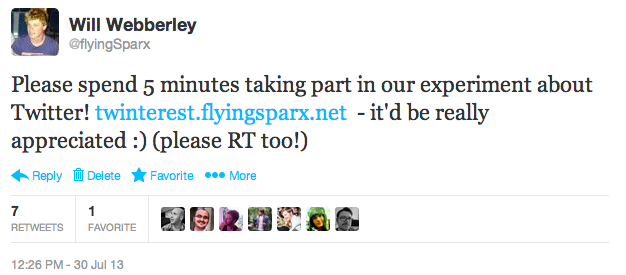
\includegraphics[scale=0.5]{5.Chapter3/Media/organic_advertising.png} 
\caption{Advertising the validation site on Twitter.}
\label{fig:organic_advertising}
\end{figure}

After signing into the read-only application\footnote{Twinterest: source available at https://github.com/flyingsparx/twinterestingness} and beginning the procedure, participants were faced with a series of ten Tweet timelines. The first consisted of the most recent 20 Tweets from the participant's home timeline, and the next nine consisted of user timelines of the participant's friends. Although the selection of friends for the nine user timelines was done at random, a slight bias was applied towards selecting friends with a higher follower count. Due to the nature of scale-free graphs, there are many vertices with few edges, and few with many edges. As such, in order to obtain a more even distribution of user influence, the weighting was necessary to ensure that the scoring mechanism could be validated against a range of users expressing a wider variety of retweet counts.

Similar to the initial validations using Mechanical Turk in the previous section, participants were simply asked to select the Tweets that they found to be the most interesting from each of the timelines and were not able to proceed to the next timeline without selecting at least one Tweet. Note that, at this stage, the Tweets being assessed did not have interestingness scores applied to them. A Tweet in a timeline that was selected was considered to be interesting, and those not selected were non-interesting.


\subsection{Assigning Scores to the Assessed Tweets}
Through running the validation application, a total of 580 timelines were assessed, consisting of 389 contributed to by MTWs and 191 from organic participants. The totals are not precisely divisible by ten since not all participants assessed all of their ten timelines before leaving the application, but no one participant contributed more than ten timeline assessments. In this case, all responses were considered as confident since it was not appropriate under the conditions of the validation test to gain more than one assessment for each Tweet. Although there was likely some friend overlap between the participants, this was not necessarily the case in the vast majority of users assessed. In cases where there the same Tweet was assessed by more than one user the majority vote was chosen, weighted towards positive interestingness decisions in the case of ties. 

\begin{figure}[h]
\centering
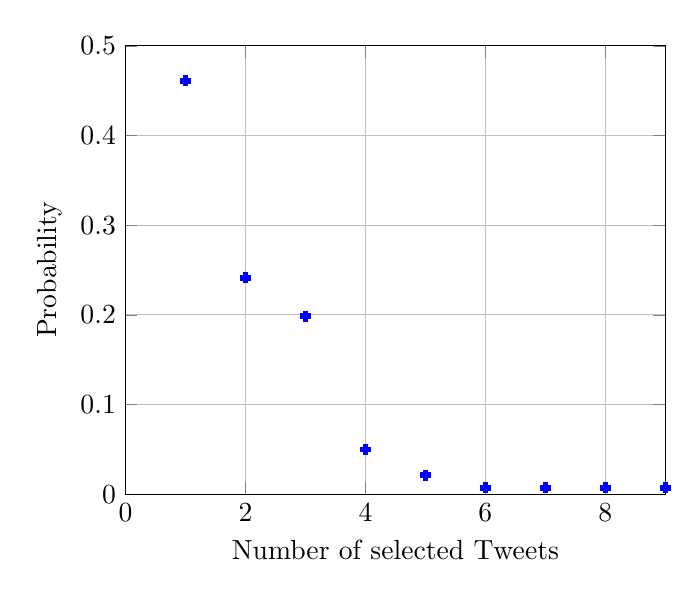
\begin{tikzpicture}
 \begin{axis}[
        xlabel=Number of selected Tweets,
        ylabel=Probability,
        grid = major,
        ymax=0.5,
        ymin=0,
        xmin=0,
        xmax=9
       ]
	\addplot[mark=+,only marks,blue]  plot coordinates {
        (1,0.460992908)(2,0.241134752)(3,0.19858156)(4,0.04964539)(5,0.021276596)(6,0.007092199)(7,0.007092199)(8,0.007092199)(9,0.007092199)
    };
\end{axis}
\end{tikzpicture}
\caption{Probability of selecting different numbers of Tweets from each timeline}
\label{fig:num_tweets_selected}

\end{figure}
The validation test resulted in a set of just under 10,000 Tweets, authored by 936 unique users, that had interestingness decisions made on them as part of the assessment of the participants' home timelines and friends' user timelines. These Tweets became the testing dataset $T$, and in order to determine their predicted expected retweet counts using trained classifiers as part of assigning the interestingness scores to each of the Tweets, two procedures were required to take place;
\begin{itemize}
    \item Collect further data on each assessed \textit{author} in order to generate the `user' models, and;
    \item Collect further data on each assessed \textit{Tweet} in order to classify it against the global model and the relevant user model.
\end{itemize}
The global model used was the same large model generated during the previous validation tests.

For privacy reasons, each participant's Twitter API credentials were not maintained by the application and so standard authenticated REST API requests were performed to collect the additional data required. In particular, in August 2013, each of the 936 users representing $\aut{t}{O} \forall t \in T$ were queried under an identical collection scheme to that used as part of the previous validation; information on the author itself and on a sample of the author's followers and friends. The collected information was also assigned to each of that user's Tweets $t' \in T$ so that an instance could be built for every $t \in T$ according to the features described in Table \ref{table:globalfeatures}. These Tweets were then classified by the global model and their appropriate user model, which was built from its author's features, in order to eventually produce the two scores. 

It should be noted that if a particular user follows another whose account is protected (see earlier in the thesis for further information on this), then the former user's API credentials can be used to view the latter's information and Tweets. However, since, during the data-collection, a static account was used to query the API, then Tweets and user information for accounts that are protected could not successfully be retrieved. This means that user and Tweet data for these users could not be collected for the purposes of training the user model and testing Tweets against this and the global model, and thus Tweets from protected authors had to be removed from $T$. The numbers stated in this section are those of the \textit{final} dataset after removing these Tweets and users.


\subsection{Results from the Further Validations}
In this section, the patterns observed through the comparison of the Tweers inferred as interesting through the scores and those indicated as interesting by the human participants are analysed. There was no significant difference observed between the accuracy of the scores against the MTWs' and the organic participants' decisions, and thus the combination both sets was considered in the following analyses.

\subsubsection{Ranking performance in further depth}
\begin{figure}[h]
\begin{subfigure}{.5\textwidth}
    \centering
    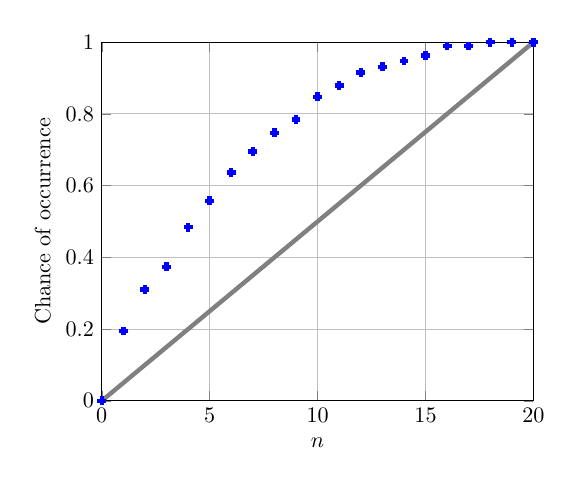
\begin{tikzpicture}[scale=0.8]
    \begin{axis}[
            ylabel=Chance of occurrence,
            xlabel=$n$,
            grid=major,
            xmin=0,
            xmax=20,
            ymin=0,
            ymax=1
            ]
       \addplot[mark=+,only marks,blue] plot coordinates{
            (0,0)(1,0.194737)(2,0.310526)(3,0.373684)(4,0.484211)(5,0.557895)(6,0.636842)(7,0.694737)(8,0.747368)(9,0.784211)(10,0.847368)(11,0.878947)(12,0.915789)(13,0.931579)(14,0.947368)(15,0.963158)(16,0.989474)(17,0.989474)(18,1)(19,1)(20,1)
        };    
        \addplot[gray] plot coordinates{
            (0,0)(1,0.05)(2,0.1)(3,0.15)(4,0.2)(5,0.25)(6,0.3)(7,0.35)(8,0.4)(9,0.45)(10,0.5)(11,0.55)(12,0.6)(13,0.65)(14,0.7)(15,0.75)(16,0.8)(17,0.85)(18,0.9)(19,0.95)(20,1) 
        }; 
    \end{axis}
    \end{tikzpicture}
    \caption{In timelines where one Tweet was selected}
    \label{fig:rank-one}
\end{subfigure}
\quad
\begin{subfigure}{.5\textwidth}
    \centering
    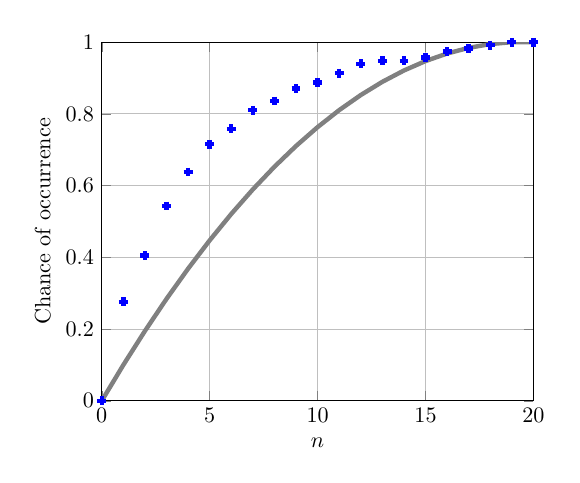
\begin{tikzpicture}[scale=0.8]
    \begin{axis}[
            ylabel=Chance of occurrence,
            xlabel=$n$,
            grid=major,
            xmin=0,
            xmax=20,
            ymin=0,
            ymax=1
            ]
       \addplot[mark=+,only marks,blue] plot coordinates{
       (0,0)(1,0.275862)(2,0.405172)(3,0.543103)(4,0.637931)(5,0.715517)(6,0.758621)(7,0.810345)(8,0.836207)(9,0.87069)(10,0.887931)(11,0.913793)(12,0.939655)(13,0.948276)(14,0.948276)(15,0.956897)(16,0.974138)(17,0.982759)(18,0.991379)(19,1)(20,1) 
        };    
        \addplot[gray] plot coordinates{
        (0,0)(1,0.1)(2,0.194736842)(3,0.284210526)(4,0.368421053)(5,0.447368421)(6,0.521052632)(7,0.589473684)(8,0.652631579)(9,0.710526316)(10,0.763157895)(11,0.810526316)(12,0.852631579)(13,0.889473684)(14,0.921052632)(15,0.947368421)(16,0.968421053)(17,0.984210526)(18,0.994736842)(19,1)(20,1)
        }; 
    \end{axis}
    \end{tikzpicture}
    \caption{In timelines where two Tweets were selected}
    \label{fig:rank-two}
\end{subfigure}
\begin{subfigure}{.5\textwidth}
    \centering
    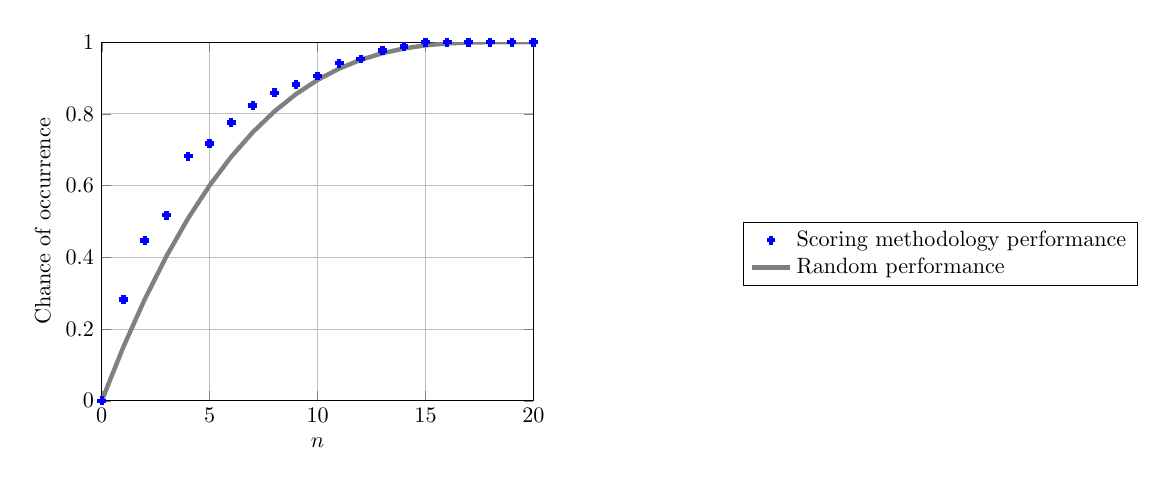
\begin{tikzpicture}[scale=0.8]
    \begin{axis}[
            ylabel=Chance of occurrence,
            xlabel=$n$,
            grid=major,
            xmin=0,
            xmax=20,
            ymin=0,
            ymax=1,
            legend entries={Scoring methodology performance, Random performance},
            legend style={at={(2.4,0.5)}, nodes={right}}
            ]
       \addplot[mark=+,only marks,blue] plot coordinates{
            (0,0)(1,0.282353)(2,0.447059)(3,0.517647)(4,0.682353)(5,0.717647)(6,0.776471)(7,0.823529)(8,0.858824)(9,0.882353)(10,0.905882)(11,0.941176)(12,0.952941)(13,0.976471)(14,0.988235)(15,1)(16,1)(17,1)(18,1)(19,1)(20,1)
        };    
        \addplot[gray] plot coordinates{
            (0,0)(1,0.15)(2,0.284210526)(3,0.403508772)(4,0.50877193)(5,0.600877193)(6,0.680701754)(7,0.749122807)(8,0.807017544)(9,0.855263158)(10,0.894736842)(11,0.926315789)(12,0.950877193)(13,0.969298246)(14,0.98245614)(15,0.99122807)(16,0.996491228)(17,0.999122807)(18,1)(19,1)(20,1)
        }; 
    \end{axis}
    \end{tikzpicture}
    \caption{In timelines where three Tweets were selected}
    \label{fig:rank-three}
\end{subfigure}
\caption{The chance of a participant selecting one of the top $n$ ranked Tweets in the timeline}
\end{figure}

In the prevoius validation, the performance of the interestingness scores in ranking Tweets was assessed on a per-question basis. The same concept is expanded here to apply a similar assessment of the scores on the present validation test.

In this case, each assessed \textit{timeline} was ranked in order of descending interestingness score in an effort to find the probability of a participant selecting a Tweet occurring in the top $n$ of Tweets. Timelines were up to 20 Tweets long, compared to the five used in the Mechanical Turk questions in the initial validation test, but the scores have again demonstrated that they are effectively able to rank Tweets. Since the timelines are bigger than the questions used before, the chance of a participant selecting multiple Tweets from a timeline was greater, as indicated by Figure \ref{fig:num_tweets_selected}. To illustrate this, the results for this analysis are demonstrated against the appropriate random performance benchmark produced by the different selection criteria. 



- chance of not selecting bottom n tweets


\section{Chapter Summary}

\subsection{Interestingness Scores}
Brief overview of scores

\subsection{Validations}
The different validations conducted

\subsection{Improvements and Qualities}
Good results, etc.
Improvements over previous methods, etc.
Works well in the general case and in more relevant situations

- remove links between users, do still receive the information - (future work?)
